\setcounter{chaptercntr}{3}

\sectionbreak {
\gostTitleFont
\redline
\thechaptercntr . 
СБОР И ПОДГОТОВКА ДАТАСЕТА ПРОДУКЦИИ САНТА ИМПЭКС
}

\subtitlespace

\subsection*{ 
  \gostTitleFont
  \redline
  \thechaptercntr .\thesubchaptercntr \spc
  Анализ и структура собираемых данных
} \addtocounter{subchaptercntr}{1}

\subtitlespace

{\gostFont

  \par \redline Ключевым условием успешного обучения модели детекции объектов является наличие качественного и представительного датасета. Поскольку специализированных открытых датасетов с изображениями продукции компании Санта Импэкс не существует, датасет для обучения модели YOLOv8n собирается самостоятельно в торговых точках, реализующих мороженое данной компании.

  \par \redline Датасет включает изображения продукции четырёх торговых марок: \textbf{ТОП}, \textbf{Soletto}, \textbf{ЮККИ} и \textbf{ТОП ЛЕД}, охватывающих различные форматы упаковки: рожки, стаканчики, эскимо, контейнеры и пакеты. Полный перечень классов SKU представлен в таблице \thechaptercntr .\thetablecntr.

  \topTablespace
  {\begin{Center}
    \par Таблица \thechaptercntr .\thetablecntr \spc {--} Классы датасета продукции Санта Импэкс.

  \begin{tabular}{|c|l|l|l|}
    \hline
    \textbf{ID} & \textbf{Бренд} & \textbf{Серия} & \textbf{Вкус / Граммовка} \\ \hline
    0  & ТОП       & Рожок           & Клубника со сливками, 75 г \\ \hline
    1  & ТОП       & Рожок           & Фисташка, 75 г \\ \hline
    2  & ТОП       & Стаканчик       & Шоколад / Ваниль, 65 г \\ \hline
    3  & ТОП       & Эскимо          & Карамель / Арахис, 70 г \\ \hline
    4  & ТОП       & ТРИО (пакет)    & Клубника-Ваниль-Шоколад, 400 г \\ \hline
    5  & Soletto   & Рожок Classico  & Лаванда-Черника, 75 г \\ \hline
    6  & Soletto   & Рожок Classico  & Фисташка-Марципан, 75 г \\ \hline
    7  & Soletto   & Рожок Classico  & Гранат-Лимон, 75 г \\ \hline
    8  & Soletto   & Gourmet (стакан)& Кедровый орех-Гауда, 190 г \\ \hline
    9  & Soletto   & Gourmet (стакан)& Шоколад-Брауни, 190 г \\ \hline
    10 & ЮККИ      & Пломбир (стакан)& На сливках (ваниль), 65 г \\ \hline
    11 & ЮККИ      & Пломбир (эскимо)& В шоколадной глазури, 70 г \\ \hline
    12 & ЮККИ      & Контейнер       & Муравейник (с маком/печеньем), 450 г \\ \hline
    13 & ЮККИ      & Семейное (пакет)& Ваниль / Шоколад, 400 г \\ \hline
    14 & ТОП ЛЕД   & Фруктовый лёд   & Малина-Лимон / Арбуз, 70 г \\ \hline
  \end{tabular} \end{Center}}
  \botTablespace \addtocounter{tablecntr}{1}

  \par \redline Итого датасет включает $N_{\mathrm{cls}} = 15$ классов объектов. С точки зрения инженерии машинного обучения необходимо оценить достаточность данных для обучения. Для обеспечения статистической репрезентативности каждого класса при обучении YOLOv8 минимально необходимое количество аннотированных объектов на класс составляет $n_{\mathrm{obj}} = 300$. Тогда минимальный объём датасета определяется по формуле (\thechaptercntr .\theformulacntr):

  \formulaspace \par \redline
    $N_{\mathrm{min}} = N_{\mathrm{cls}} \times n_{\mathrm{obj}} = 15 \times 300 = 4500 \text{ объектов}$
    \hfill (\thechaptercntr .\theformulacntr) \redline
  \formulaspace \addtocounter{formulacntr}{1}

  \par \redline Изображения для датасета собираются непосредственно в торговых точках при реальных условиях эксплуатации. Для обеспечения достаточного разнообразия обучающей выборки съёмка производится в различных условиях: при разном освещении (дневное освещение торгового зала, искусственный свет холодильного оборудования), под разными углами (фронтальный, под углом $15$–$30°$ к плоскости полки), при различной степени заполненности полок и в разных торговых точках. Такой подход позволяет повысить обобщающую способность обученной модели.

  \par \redline С точки зрения качества данных собираемый датасет обладает следующими характеристиками. Данные являются информативными, поскольку отражают реальные условия работы мерчендайзера. Данные соответствуют реальным входным данным системы: модель будет обучаться на изображениях, аналогичных тем, которые будут поступать от камеры мобильного устройства в процессе эксплуатации. Данные охватывают все классы продукции, представленные в ассортиментной матрице Санта Импэкс.

  \par \redline Для дальнейшего описания процесса сбора и анализа данных необходима их визуализация. Пример собранных изображений различных SKU продукции Санта Импэкс на полках холодильного оборудования представлен на рисунке \thechaptercntr .\theimagecntr.

  \begin{figure}[H]
    \centering
    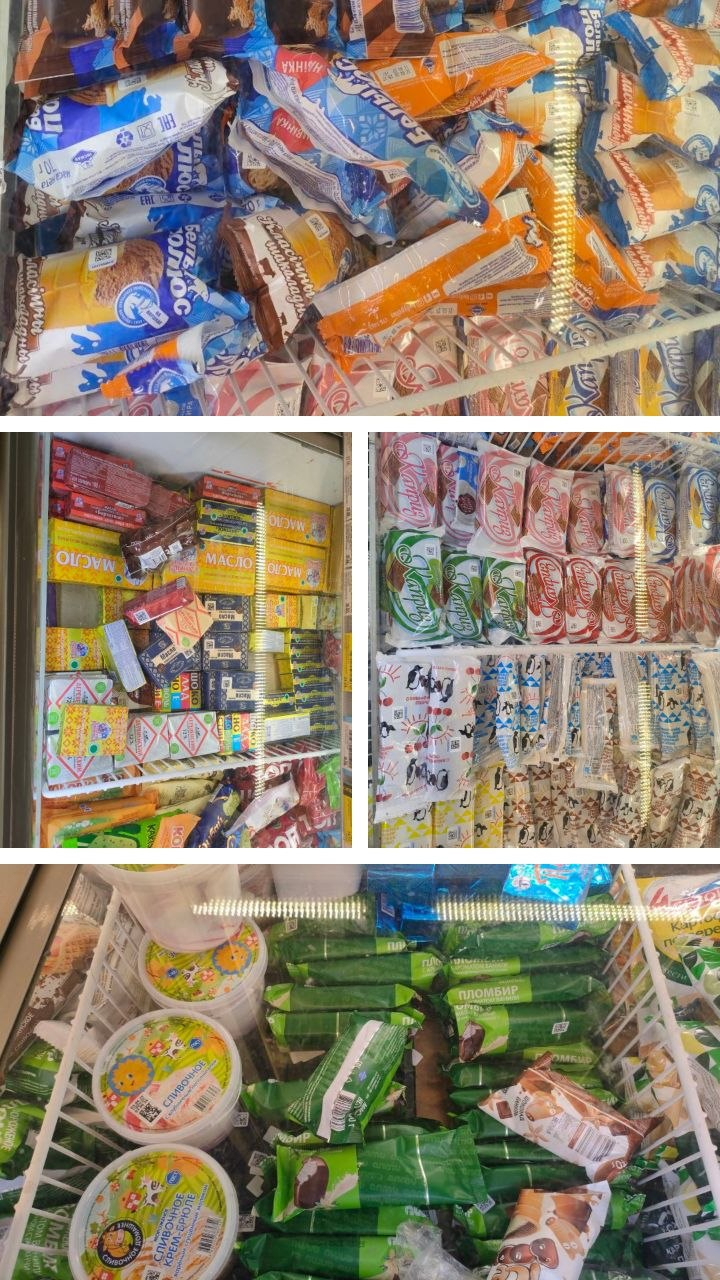
\includegraphics[width=0.8\textwidth, height=145mm]{images/dataset_raw_samples.png}
    \caption*{\gostFont Рисунок \thechaptercntr .\theimagecntr \spc {--} Примеры изображений из собранного датасета продукции Санта Импэкс.}
    \label{fig:dataset_raw}
  \end{figure} \addtocounter{imagecntr}{1}

  \par \redline Анализ собранных изображений позволяет выявить ряд характерных сложностей, которые необходимо учесть при подготовке датасета и настройке модели. Во-первых, ряд SKU имеют схожую цветовую гамму упаковки (например, рожок ТОП «Клубника со сливками» и рожок Soletto «Гранат-Лимон» содержат красно-розовые оттенки), что потенциально ведёт к смешению классов. Во-вторых, упаковки в формате пакетов (ТОП ТРИО, ЮККИ Семейное) существенно отличаются по размеру от штучных позиций, что влияет на выбор масштаба детекции. В-третьих, часть позиций может быть частично перекрыта другими упаковками или ценниками, что создаёт сложные условия для детекции.

  \par \redline Также важно отметить отсутствие данных с аномальными условиями съёмки: размытые изображения, слишком тёмные или засвеченные кадры, изображения с нехарактерными углами съёмки исключаются из датасета на этапе первичной фильтрации. Это позволяет обеспечить высокое качество обучающей выборки.

  \par
}

\subtitlespace

\subsection*{
  \gostTitleFont
  \redline
  \thechaptercntr .\thesubchaptercntr \spc
  Разметка данных и формирование датасета
} \addtocounter{subchaptercntr}{1}

\subtitlespace

{\gostFont

  \par \redline После сбора изображений необходимо выполнить их аннотирование (разметку) — процесс ручной разметки объектов на каждом изображении с указанием координат ограничивающих прямоугольников (bounding boxes) и соответствующих меток классов. Разметка выполняется с использованием платформы \textbf{Roboflow}, предоставляющей удобный веб-интерфейс для аннотирования изображений и управления датасетом.
  \par \redline Формат YOLO использует нормализованные координаты, что обеспечивает независимость разметки от разрешения исходного изображения. Каждая строка текстового файла аннотации включает в себя индекс класса и четыре вещественных числа: координаты центра ограничивающего прямоугольника ($x, y$), а также его ширину ($w$) и высоту ($h$). Значения координат варьируются в диапазоне от 0 до 1, где начало отсчета находится в верхнем левом углу изображения. Такая система представления данных позволяет эффективно подавать изображения разных размеров на вход нейронной сети без необходимости пересчета координат вручную.

  \par \redline В процессе разметки особое внимание уделяется точности позиционирования рамок и полноте охвата объектов. Для проекта «Retail Vision» критически важным является исключение фрагментарных перекрытий, когда один объект может быть ошибочно принят за несколько разных. Использование инструментов Roboflow позволяет автоматизировать часть рутинных операций, например, через применение функций интеллектуального выделения контуров или копирования разметки для схожих ракурсов, что существенно ускоряет подготовку массива данных объемом в несколько сотен или тысяч экземпляров.

  \par \redline Завершающим этапом подготовки является верификация аннотаций, направленная на выявление и исправление ошибок человеческого фактора: пропущенных объектов, неверно назначенных классов или избыточно широких границ рамок. Качественно размеченный датасет выступает фундаментом для обучения модели, так как наличие шума в обучающей выборке напрямую коррелирует с увеличением функции потерь и снижением метрик средней точности ($mAP$) при последующем тестировании системы.
  \par \redline Аннотации хранятся в стандартном для YOLO текстовом формате. Каждому изображению соответствует текстовый файл с расширением \texttt{.txt}, содержащий одну строку на каждый аннотированный объект в следующем виде:

  \formulaspace
  \begin{Center}
    \texttt{<class\_id> <x\_c> <y\_c> <w> <h>}
  \end{Center}
  \formulaspace

  \begin{tabular}{p{0,875cm}p{0,3cm}p{15,175cm}}
      & где  & \texttt{class\_id} {--} целочисленный идентификатор класса объекта (от 0 до 14); \\
      &      & \texttt{x\_c}, \texttt{y\_c} {--} нормализованные координаты центра ограничивающего прямоугольника относительно ширины и высоты изображения соответственно; \\
      &      & \texttt{w}, \texttt{h} {--} нормализованные ширина и высота ограничивающего прямоугольника. \\
  \end{tabular}

  \par \redline Нормализация координат производится по формулам (\thechaptercntr .\theformulacntr):

  \formulaspace \par \redline
    $x_c = \scaleto{\frac{x_{\mathrm{left}} + x_{\mathrm{right}}}{2 \cdot W_{\mathrm{img}}}}{24pt}, \quad y_c = \scaleto{\frac{y_{\mathrm{top}} + y_{\mathrm{bottom}}}{2 \cdot H_{\mathrm{img}}}}{24pt}$
    \hfill (\thechaptercntr .\theformulacntr) \redline
  \formulaspace \addtocounter{formulacntr}{1}

  \begin{tabular}{p{0,875cm}p{0,3cm}p{15,175cm}}
      & где  & $x_{\mathrm{left}},\, x_{\mathrm{right}}$ {--} пиксельные координаты левой и правой границ объекта; \\
      &      & $y_{\mathrm{top}},\, y_{\mathrm{bottom}}$ {--} пиксельные координаты верхней и нижней границ объекта; \\
      &      & $W_{\mathrm{img}},\, H_{\mathrm{img}}$ {--} ширина и высота изображения в пикселях. \\
  \end{tabular}

  \par \redline Все значения нормализованных координат принадлежат диапазону $[0;\,1]$, что обеспечивает независимость формата аннотаций от разрешения изображений. Пример размеченного изображения с ограничивающими прямоугольниками и метками классов показан на рисунке \thechaptercntr .\theimagecntr.

  \begin{figure}[H]
    \centering
    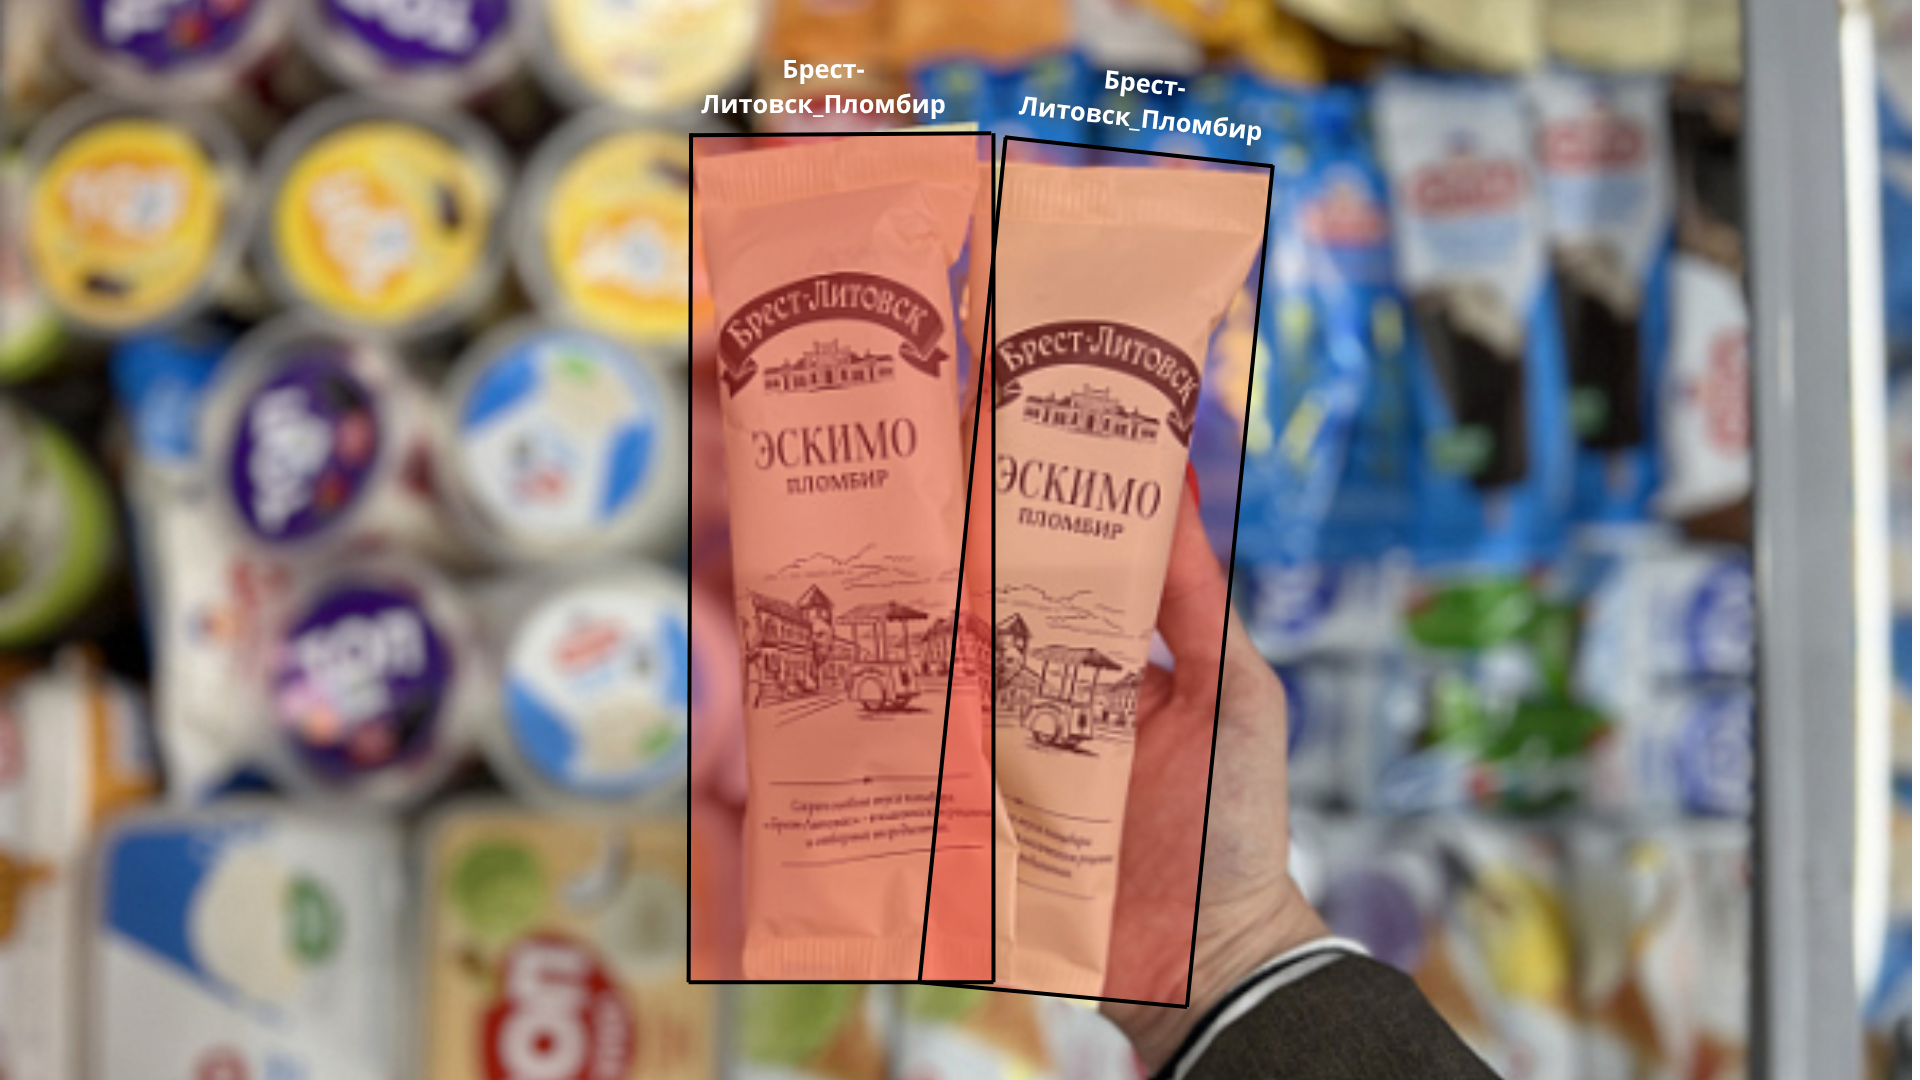
\includegraphics[width=\textwidth]{images/dataset_annotation_example.png}
    \caption*{\gostFont Рисунок \thechaptercntr .\theimagecntr \spc {--} Пример аннотированного изображения продукции Санта Импэкс с ограничивающими прямоугольниками.}
    \label{fig:annotation}
  \end{figure} \addtocounter{imagecntr}{1}

  \par \redline Итоговый датасет разбивается на три подмножества в соответствии с требованиями инженерии машинного обучения. \textbf{Обучающая выборка} используется непосредственно для обновления весовых коэффициентов модели в процессе обучения. \textbf{Валидационная выборка} служит для оценки качества модели после каждой эпохи обучения и подбора гиперпараметров. \textbf{Тестовая выборка} используется для финальной оценки обученной модели на данных, не участвовавших ни в обучении, ни в валидации. Соотношение выборок составляет 70\% / 15\% / 15\% соответственно.

  \par \redline Структура директорий датасета в формате Ultralytics YOLOv8 организована следующим образом:

  \formulaspace
  \begin{Center}
    \texttt{dataset/ images/train/, images/val/, images/test/}
    
    \texttt{dataset/ labels/train/, labels/val/, labels/test/}
  \end{Center}
  \formulaspace

  \par \redline Конфигурационный файл датасета \texttt{data.yaml} содержит пути к директориям, количество классов 
  и их имена. Этот файл передаётся модели YOLOv8 при запуске обучения.

  \par \redline Для обеспечения равномерного распределения классов в выборках используется стратифицированное 
  разбиение датасета. Распределение количества аннотированных объектов по классам показано на 
  рисунке \thechaptercntr .\theimagecntr.
  \par \redline Анализ представленной ниже гистограммы позволяет оценить степень дисбаланса классов, который является характерной особенностью прикладных задач компьютерного зрения в ритейле. Неравномерность распределения объектов обусловлена естественными различиями в представленности конкретных товарных позиций на торговых полках, а также вариативностью спроса на отдельные виды продукции. Визуализация данной проблемы непосредственно в условиях торговой точки представлена на рисунке \thechaptercntr.\theimagecntr.

  % ВСТАВКА НОВОГО РИСУНКА
  \begin{figure}[H]
    \centering
    % Масштабируем по ширине текста, сохраняя пропорции
    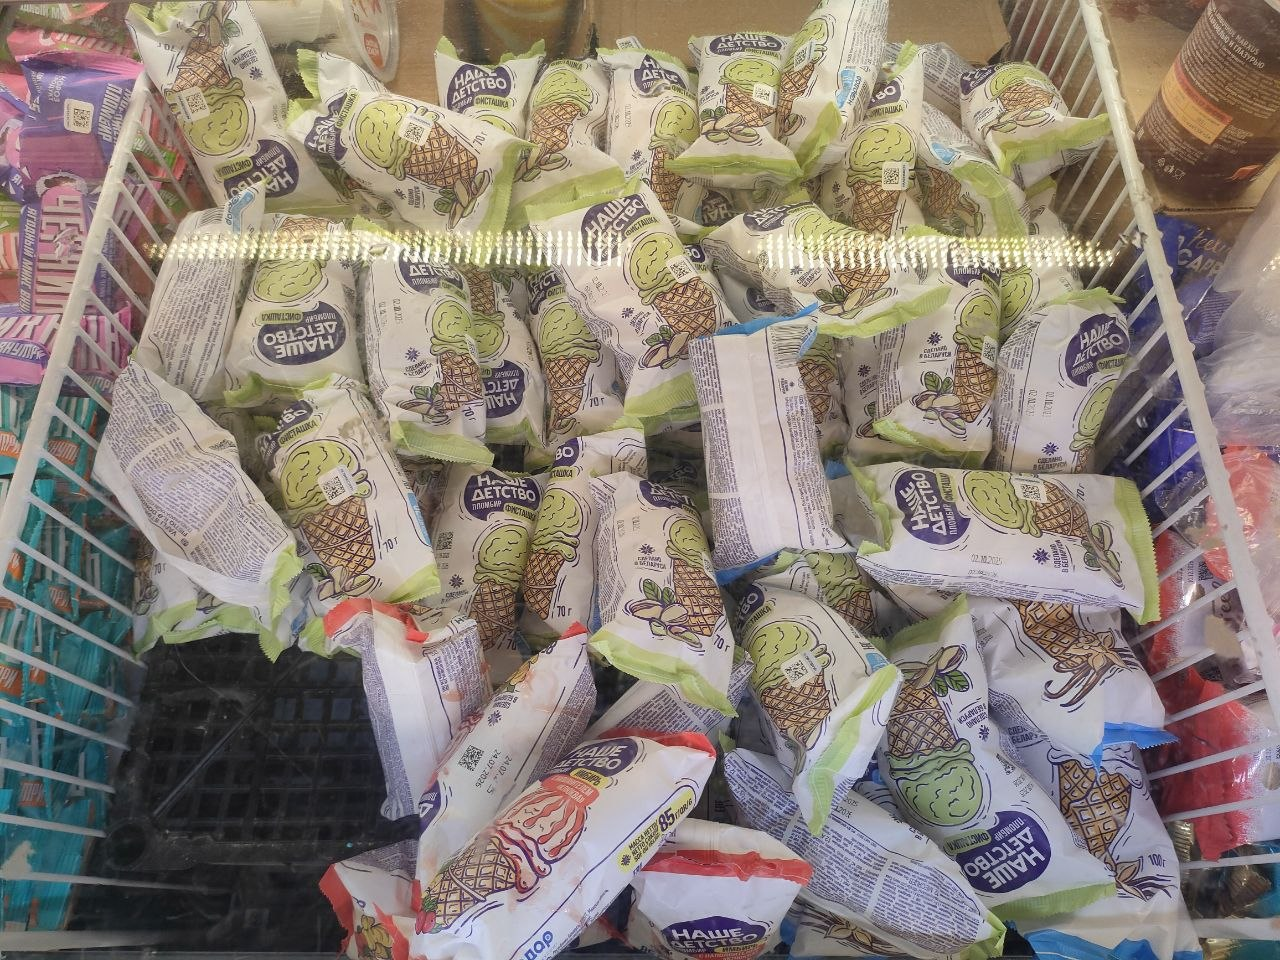
\includegraphics[width=0.8\textwidth]{images/shelf_class_imbalance_visual.png}
    \caption*{\gostFont Рисунок \thechaptercntr.\theimagecntr\spc {--} Визуализация дисбаланса классов на примере выкладки продукции: доминирование мажоритарного SKU над миноритарными.}
    \label{fig:imbalance_visual}
  \end{figure}
  \addtocounter{imagecntr}{1} % Увеличиваем счетчик после отрисовки

  \par \redline На изображении отчетливо видно, что мажоритарные классы (выделены красным цветовым тоном) занимают фейсинг, 
  в несколько раз превосходящий площадь, отведенную под редкие SKU (выделены синим). Учет данной специфики на этапе подготовки 
  данных критически важен для предотвращения смещения модели в сторону доминирующих позиций. В противном случае, нейронная сеть 
  будет демонстрировать высокую точность на частых объектах, игнорируя или ошибочно классифицируя редкие, но критически важные 
  для аналитики позиции, что приведет к существенному снижению метрик mAP при тестировании системы.
  Для минимизации подобных рисков в работе применяется комплексный подход, включающий не только стратификацию выборки, но и использование 
  специализированных функций потерь, таких как Focal Loss, которые позволяют динамически перевзвешивать вклад каждого примера в процесс 
  обучения.
   \begin{figure}[H]
  \centering
  \rotatebox{90}{%
    % Задаем ширину минипейджа равной высоте текстового поля страницы
    \begin{minipage}{0.9\textheight} 
      \centering
      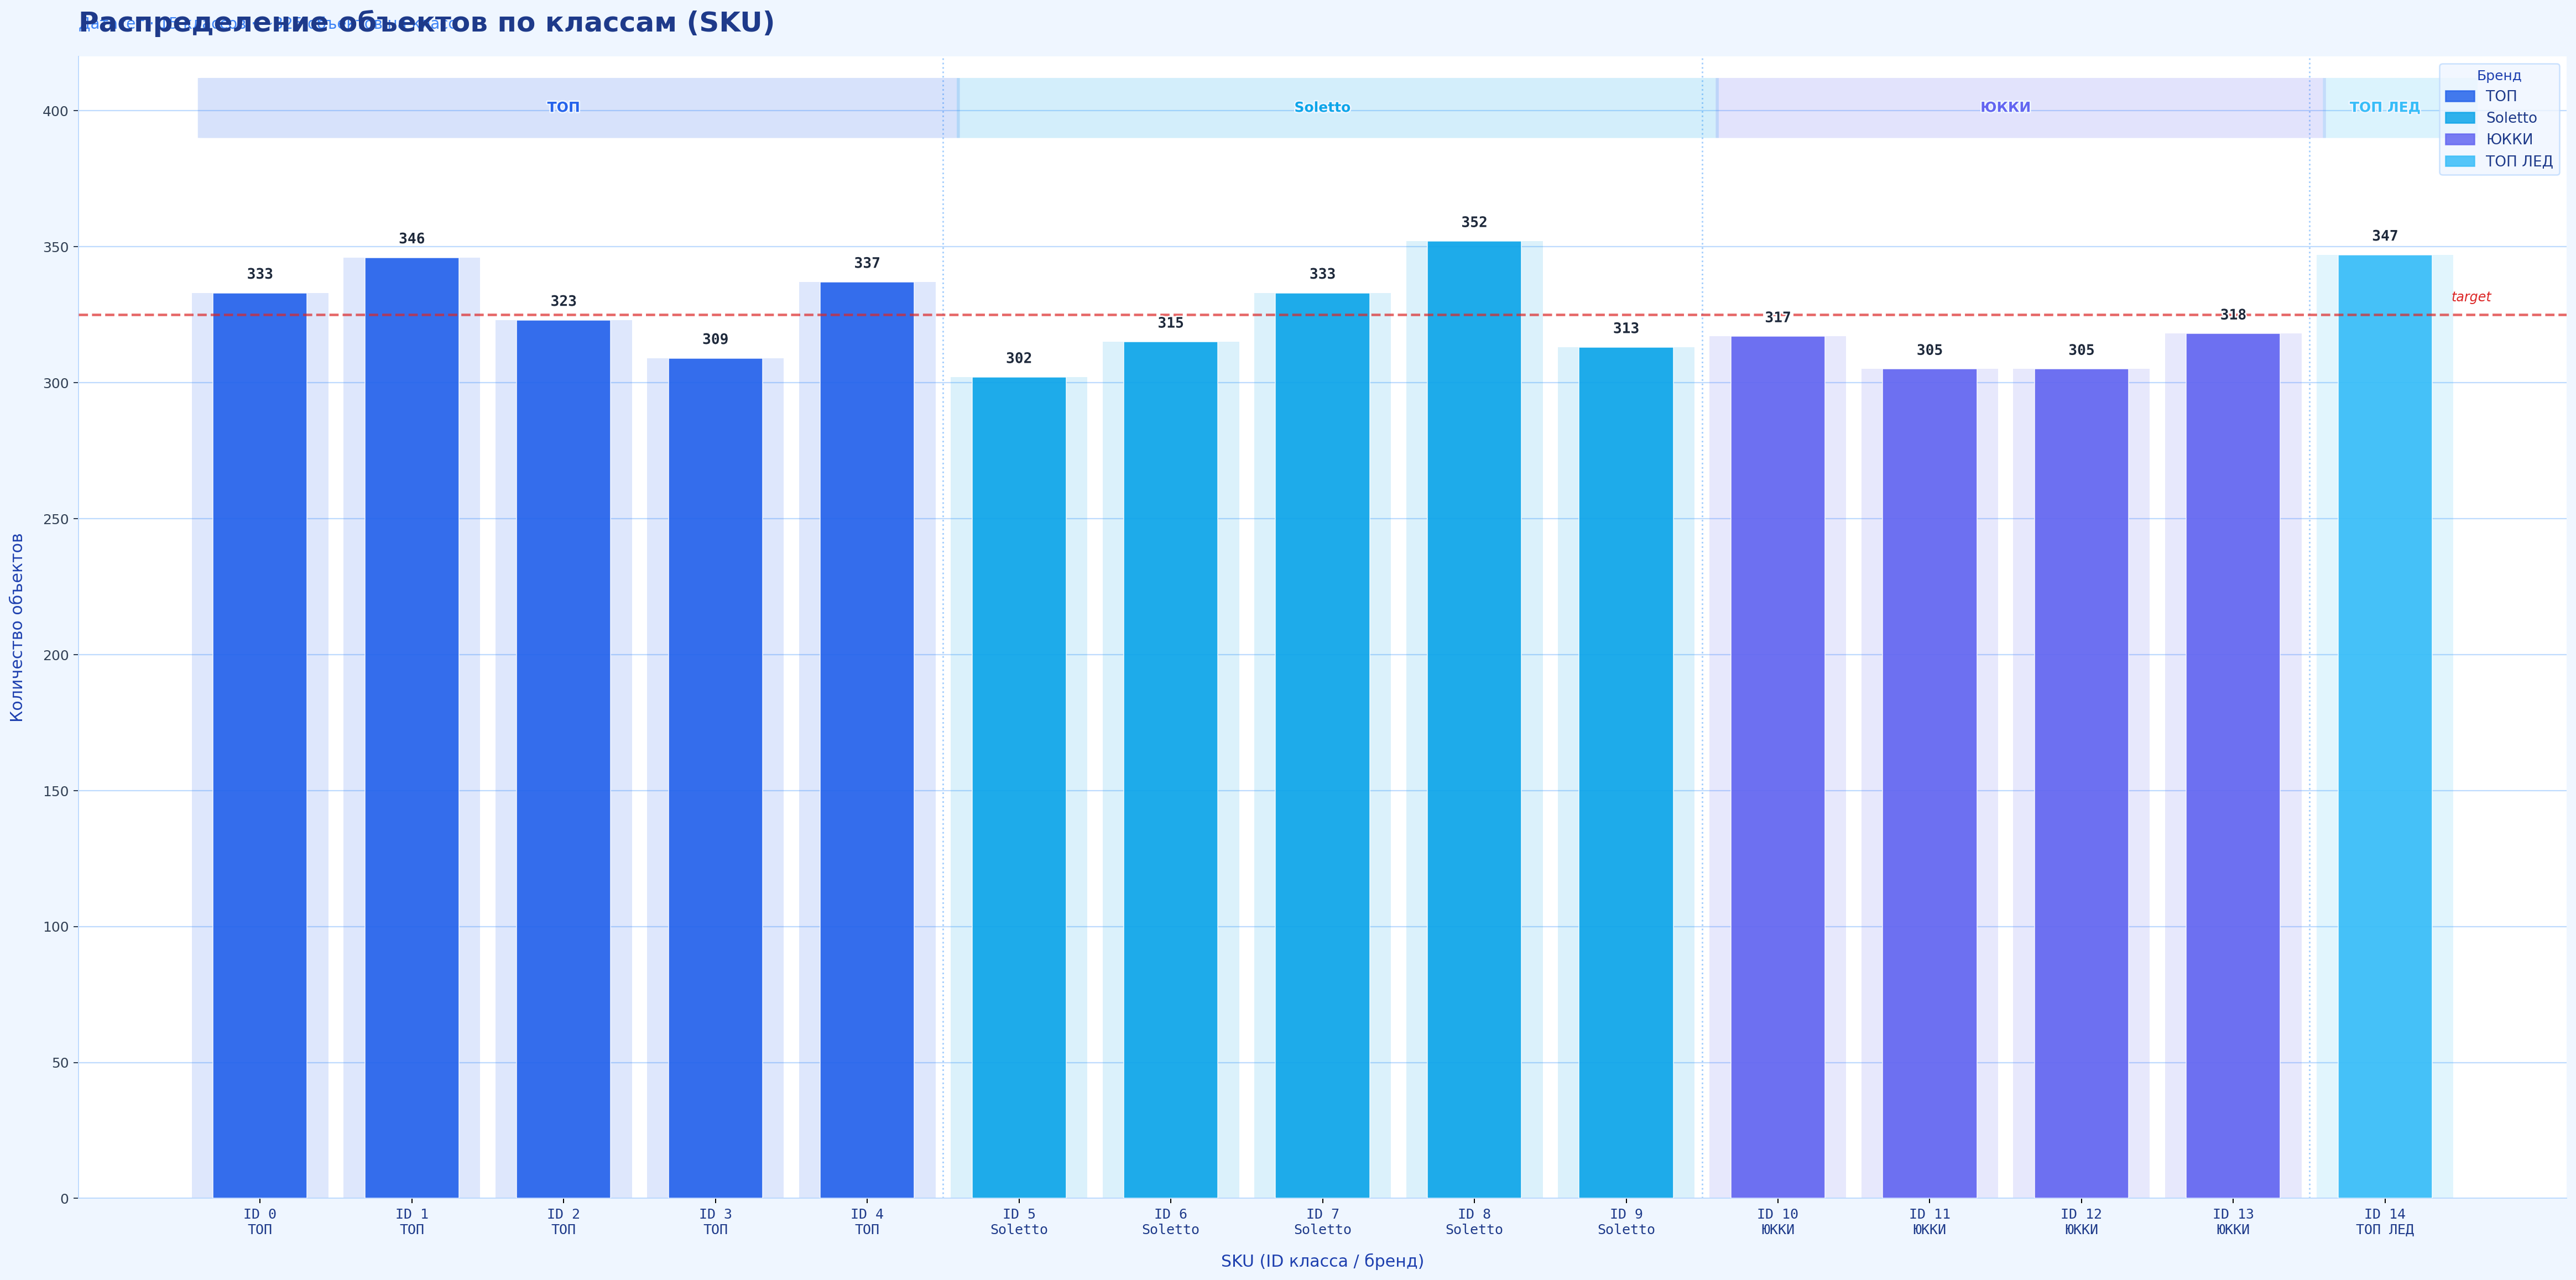
\includegraphics[width=\textwidth, keepaspectratio]{images/dataset_class_distribution.png}
      \vspace{2mm} % Небольшой отступ между картинкой и подписью
      \caption*{\gostFont Рисунок \thechaptercntr.\theimagecntr\spc {--} Распределение количества объектов по классам в датасете.}
      \label{fig:class_dist}
    \end{minipage}%
  }
\end{figure}
\addtocounter{imagecntr}{1}
  \par
}

\subtitlespace

\subsection*{
  \gostTitleFont
  \redline
  \thechaptercntr .\thesubchaptercntr \spc
  Обработка данных и аугментация
} \addtocounter{subchaptercntr}{1}

\subtitlespace

{\gostFont

  \par \redline После первичного сбора и разметки изображений необходимо выполнить их обработку и подготовку к обучению модели. Основными задачами данного этапа являются нормализация изображений, их масштабирование до входного размера модели и аугментация данных с целью расширения обучающей выборки и повышения обобщающей способности модели.

  \par \redline Первым шагом предобработки является масштабирование изображений до стандартного входного размера YOLOv8 $640 \times 640$ пикселей. Поскольку исходные изображения, снятые камерой смартфона, имеют различные разрешения и соотношения сторон, применяется метод \textbf{letterbox-масштабирования}: изображение пропорционально уменьшается до тех пор, пока его большая сторона не достигнет 640 пикселей, а оставшееся пространство заполняется серыми полосами. Это исключает искажение пропорций объектов. Пересчёт координат аннотаций при letterbox-масштабировании выполняется по формуле (\thechaptercntr .\theformulacntr):

  \formulaspace \par \redline
    $s = \scaleto{\frac{imgsz}{\max(W_{\mathrm{img}},\, H_{\mathrm{img}})}}{22pt}$
    \hfill (\thechaptercntr .\theformulacntr) \redline
  \formulaspace \addtocounter{formulacntr}{1}

  \begin{tabular}{p{0,875cm}p{0,3cm}p{15,175cm}}
      & где  & $s$ {--} коэффициент масштабирования; \\
      &      & $imgsz = 640$ {--} целевой размер входного изображения. \\
  \end{tabular}

  \par \redline Нормализация значений пикселей выполняется делением на 255 для приведения диапазона значений из $[0;\,255]$ к диапазону $[0;\,1]$ по формуле (\thechaptercntr .\theformulacntr):

  \formulaspace \par \redline
    $\hat{p} = \scaleto{\frac{p}{255}}{22pt}$
    \hfill (\thechaptercntr .\theformulacntr) \redline
  \formulaspace \addtocounter{formulacntr}{1}

  \begin{tabular}{p{0,875cm}p{0,3cm}p{15,175cm}}
      & где  & $p \in [0;\,255]$ {--} исходное значение пикселя; \\
      &      & $\hat{p} \in [0;\,1]$ {--} нормализованное значение пикселя. \\
  \end{tabular}

  \par \redline Аугментация данных является ключевым инструментом расширения обучающей выборки и снижения риска переобучения модели. В пайплайне обучения YOLOv8 применяются следующие виды аугментации.

  \par \redline \textbf{HSV-аугментация} — случайное изменение тона (Hue), насыщенности (Saturation) и яркости (Value) изображения в заданных диапазонах. Это моделирует различные условия освещения в торговых точках. Параметры: $\Delta H \in [-0{,}015;\, 0{,}015]$, $\Delta S \in [0{,}7;\, 1{,}3]$, $\Delta V \in [0{,}4;\, 1{,}6]$.

  \par \redline \textbf{Горизонтальное отражение} (horizontal flip) — симметричное отражение изображения относительно вертикальной оси с вероятностью $p = 0{,}5$. При этом координаты аннотаций пересчитываются по формуле (\thechaptercntr .\theformulacntr):

  \formulaspace \par \redline
    $x_c' = 1 - x_c$
    \hfill (\thechaptercntr .\theformulacntr) \redline
  \formulaspace \addtocounter{formulacntr}{1}

  \par \redline \textbf{Mosaic-аугментация} — объединение четырёх случайно выбранных изображений обучающей выборки в одно изображение $640 \times 640$ пикселей с произвольной точкой объединения. Данный вид аугментации позволяет модели обучаться на частично видимых объектах и объектах, расположенных у краёв изображения, что характерно для реальных условий съёмки полок.

  \par \redline \textbf{MixUp-аугментация} — наложение двух изображений с весовым коэффициентом $\lambda \in [0;\,1]$, определяемым из бета-распределения. Результирующее изображение вычисляется по формуле (\thechaptercntr .\theformulacntr):

  \formulaspace \par \redline
    $I_{\mathrm{mix}} = \lambda \cdot I_1 + (1 - \lambda) \cdot I_2$
    \hfill (\thechaptercntr .\theformulacntr) \redline
  \formulaspace \addtocounter{formulacntr}{1}

  \begin{tabular}{p{0,875cm}p{0,3cm}p{15,175cm}}
      & где  & $I_1,\, I_2$ {--} исходные изображения из обучающей выборки; \\
      &      & $\lambda$ {--} коэффициент смешивания, $\lambda \sim \mathrm{Beta}(\alpha,\, \alpha)$, $\alpha = 0{,}32$. \\
  \end{tabular}

  \par \redline Случайное масштабирование и кадрирование (Scale and Crop) дополнительно обеспечивает вариативность размеров объектов в обучающей выборке. Коэффициент масштабирования задаётся в диапазоне $scale \in [0{,}5;\, 1{,}5]$. Пример результатов mosaic-аугментации показан на рисунке \thechaptercntr .\theimagecntr.

  \begin{figure}[H]
    \centering
    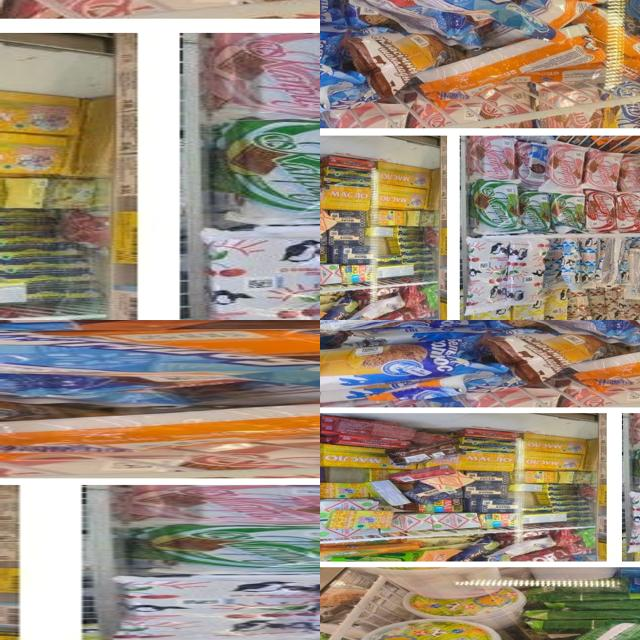
\includegraphics[width=0.8\textwidth]{images/augmentation_mosaic_example.png}
    \caption*{\gostFont Рисунок \thechaptercntr .\theimagecntr \spc {--} Пример mosaic-аугментации изображений датасета.}
    \label{fig:mosaic}
  \end{figure} \addtocounter{imagecntr}{1}

  \par \redline Учитывая особенности продукции Санта Импэкс, вертикальное отражение (vertical flip) в пайплайне аугментации \textbf{не применяется}: рожки, стаканчики и эскимо имеют строго определённую ориентацию на полке (вертикальное расположение), и перевёрнутые изображения не соответствуют реальным условиям съёмки. Это является важным отличием от типовых конфигураций аугментации и позволяет избежать обучения модели на нереалистичных данных.

  \par \redline Таким образом, применённый комплекс аугментаций позволяет существенно расширить эффективный объём обучающей выборки и обеспечить устойчивость обученной модели к вариациям условий съёмки в реальных торговых точках.

  \par
}

\setcounter{subchaptercntr}{1}
\setcounter{formulacntr}{1}
\setcounter{imagecntr}{1}
\setcounter{tablecntr}{1}